% G2-4 Pohon biasa vs pohon simetris (oblivious) CatBoost.
% Sumber: diadaptasi dari prokhorenkova2018 (hlm. PDF 6).
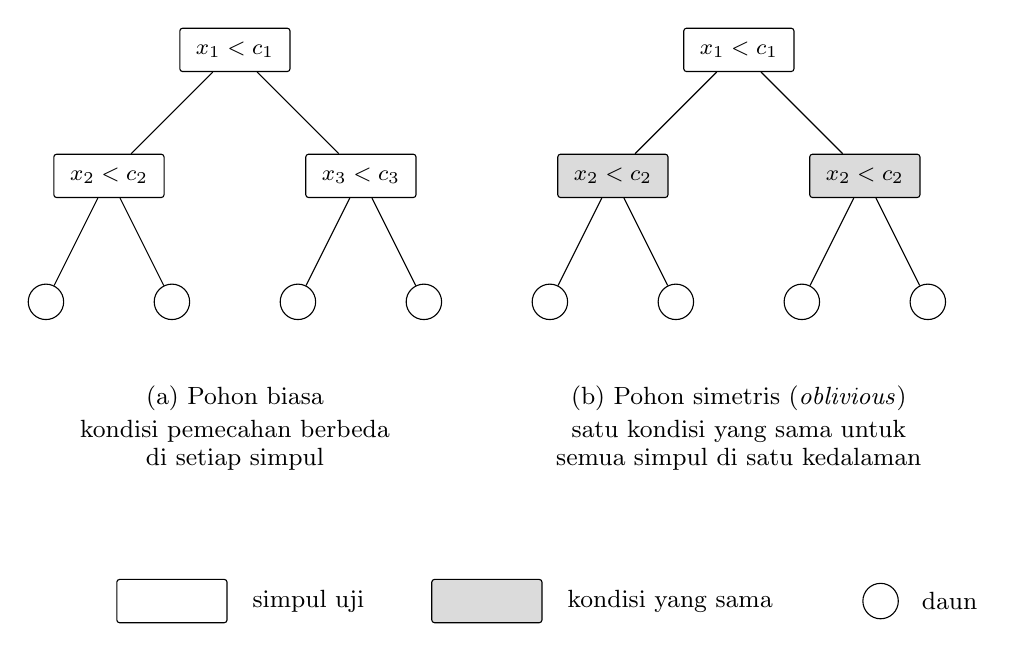
\begin{tikzpicture}[x=1mm,y=-1mm,font=\footnotesize,
    uji/.style={draw,rectangle,rounded corners=1pt,inner sep=1.5pt,
      minimum width=14mm,minimum height=5.5mm},
    sama/.style={uji,fill=black!14},
    daun/.style={draw,circle,inner sep=0pt,minimum size=4.5mm}]

  % --- panel kiri: pohon biasa, kondisi berbeda tiap simpul ---
  \begin{scope}
    \node[uji]  (a) at (30,0)  {$x_1 < c_1$};
    \node[uji]  (b) at (14,16) {$x_2 < c_2$};
    \node[uji]  (c) at (46,16) {$x_3 < c_3$};
    \node[daun] (d) at (6,32)  {};
    \node[daun] (e) at (22,32) {};
    \node[daun] (f) at (38,32) {};
    \node[daun] (g) at (54,32) {};
    \draw (a) -- (b) (a) -- (c) (b) -- (d) (b) -- (e) (c) -- (f) (c) -- (g);
    \node[font=\small,align=center] at (30,48)
      {(a) Pohon biasa\\[1pt]
       kondisi pemecahan berbeda\\[-1pt] di setiap simpul};
  \end{scope}

  % --- panel kanan: pohon simetris, satu kondisi per kedalaman ---
  \begin{scope}[xshift=64mm]
    \node[uji]  (a2) at (30,0)  {$x_1 < c_1$};
    \node[sama] (b2) at (14,16) {$x_2 < c_2$};
    \node[sama] (c2) at (46,16) {$x_2 < c_2$};
    \node[daun] (d2) at (6,32)  {};
    \node[daun] (e2) at (22,32) {};
    \node[daun] (f2) at (38,32) {};
    \node[daun] (g2) at (54,32) {};
    \draw (a2) -- (b2) (a2) -- (c2) (b2) -- (d2) (b2) -- (e2)
          (c2) -- (f2) (c2) -- (g2);
    \node[font=\small,align=center] at (30,48)
      {(b) Pohon simetris (\textit{oblivious})\\[1pt]
       satu kondisi yang sama untuk\\[-1pt]
       semua simpul di satu kedalaman};
  \end{scope}

  % --- legenda ---
  \node[uji]  at (22,70) {};
  \node[anchor=west,font=\small] at (31,70) {simpul uji};
  \node[sama] at (62,70) {};
  \node[anchor=west,font=\small] at (71,70) {kondisi yang sama};
  \node[daun] at (112,70) {};
  \node[anchor=west,font=\small] at (116,70) {daun};
\end{tikzpicture}
